\documentclass{article}
\usepackage{amsmath,amssymb}
\usepackage{graphicx}
\usepackage{geometry}
\usepackage{enumitem}
\usepackage{microtype}
\usepackage{titlesec}
\usepackage[normalem]{ulem} % for single/double underlines
\usepackage{tikz}
\usetikzlibrary{angles,quotes,arrows.meta,calc,intersections,positioning,decorations.markings}
\geometry{a4paper, margin=1in}

% Colors and typography theme (academic, readable on white)
\usepackage{xcolor}
\definecolor{primary}{HTML}{0B5394}    % deep blue
\definecolor{secondary}{HTML}{38761D}  % deep green
\definecolor{accent}{HTML}{990000}     % dark red
\definecolor{darktext}{HTML}{222222}
\color{darktext}

% Section heading styles
\titleformat*{\section}{\Large\bfseries\color{primary}}
\titleformat*{\subsection}{\large\bfseries\color{secondary}}

% Compact, colored, step-by-step lists
\newenvironment{steps}{% 
  \begin{enumerate}[label=\textcolor{primary}{Step~\arabic*:}, leftmargin=*]
}{\end{enumerate}}

% Underline helpers
\newcommand{\sul}[1]{\uline{#1}}
\newcommand{\dul}[1]{\uuline{#1}}
% Single-line Solution heading without justification to avoid underfull hbox
\newcommand{\solutionheading}{{\raggedright\dul{\textbf{Solution}}\par}}

% Callouts (underline styles: Given/Answer double, To Prove single)
\newcommand{\given}[1]{\noindent\textbf{\textcolor{secondary}{\dul{Given:}}}~#1\\}
\newcommand{\toprove}[1]{\noindent\textbf{\textcolor{primary}{\sul{To Prove:}}}~#1\\}
\newcommand{\construction}[1]{\noindent\textbf{\textcolor{secondary}{Construction:}}~#1\\}
\newcommand{\reason}[1]{\hfill\textit{\textcolor{gray}{(#1)}}}

% Boxed work highlights
\newcommand{\workbox}[1]{\fcolorbox{primary!60!black}{primary!5}{\strut\,\ensuremath{#1}\,}}

% Final answer label and end-of-solution rule
\newcommand{\solutionrule}{\par\noindent\color{accent}\rule{\linewidth}{0.6pt}\par\smallskip}
\newcommand{\finalanswer}[1]{\noindent\textbf{\textcolor{accent}{\dul{Answer:}}}~#1\solutionrule}

% Spacing for readability
\setlength{\parskip}{6pt}
\setlength{\parindent}{0pt}
\linespread{1.05}

% Hyperlinks with themed colors
\usepackage[hidelinks]{hyperref}
\hypersetup{colorlinks=true, linkcolor=primary, urlcolor=accent, citecolor=secondary}

\begin{document}

\section*{Exercise 15A Solutions}

\subsection*{Question 2}
\textbf{Question:} In triangles ABC and DEF, $\angle A = \angle D$ and $\frac{AB}{DE} = \frac{AC}{DF}$. Prove that $\triangle ABC \sim \triangle DEF$.

\solutionheading
\given{$\angle A = \angle D$ and $\dfrac{AB}{DE} = \dfrac{AC}{DF}$.}
\toprove{$\triangle ABC \sim \triangle DEF$ (SAS).}

\begin{center}
\begin{tikzpicture}[scale=1]
  % Triangle ABC
  \coordinate (A) at (0,0);
  \coordinate (B) at (3,0.6);
  \coordinate (C) at (1.2,2.2);
  \draw (A)--(B)--(C)--cycle;
  \node[below left] at (A) {A};
  \node[below right] at (B) {B};
  \node[above] at (C) {C};
  % Mark angle A
  \pic [draw, angle radius=7mm] {angle=B--A--C};
  % Triangle DEF
  \coordinate (D) at (5.2,0);
  \coordinate (E) at (8.0,0.3);
  \coordinate (F) at (6.6,2.0);
  \draw (D)--(E)--(F)--cycle;
  \node[below] at (D) {D};
  \node[below right] at (E) {E};
  \node[above] at (F) {F};
  % Mark angle D equal to A
  \pic [draw, angle radius=7mm] {angle=E--D--F};
  % Indicate proportional including sides with ticks
  \draw[decorate,decoration={markings,mark=at position 0.5 with {\draw (-2pt,0)--(2pt,0);}}] (A)--(B);
  \draw[decorate,decoration={markings,mark=at position 0.5 with {\draw (-2pt,0)--(2pt,0);}}] (D)--(E);
  \draw[decorate,decoration={markings,mark=at position 0.5 with {\draw (-2pt,0)--(2pt,0);}}] (A)--(C);
  \draw[decorate,decoration={markings,mark=at position 0.5 with {\draw (-2pt,0)--(2pt,0);}}] (D)--(F);
\end{tikzpicture}
\end{center}

\begin{steps}
  \item Identify the included angle and sides: in $\triangle ABC$, sides $AB,AC$ include $\angle A$; in $\triangle DEF$, sides $DE,DF$ include $\angle D$.\reason{definition of included angle}
  \item Use the data $\angle A=\angle D$ and $\dfrac{AB}{DE}=\dfrac{AC}{DF}$.\reason{given}
  \item Conclude $\triangle ABC\sim\triangle DEF$.\reason{SAS similarity}
\end{steps}

\finalanswer{$\triangle ABC \sim \triangle DEF$ by SAS.}

\subsection*{Question 3}
\textbf{Question:} In $\triangle ABC$ and $\triangle DEF$, $\angle A = \angle D$, $\angle B = \angle E$ and $\angle C = \angle F$. Also, AL and DM are medians. Prove that $\frac{BC}{EF} = \frac{AL}{DM}$.

\solutionheading
\given{$\triangle ABC \sim \triangle DEF$ (AAA), and $AL, DM$ are medians.}
\toprove{$\dfrac{BC}{EF} = \dfrac{AL}{DM}$.}

\begin{center}
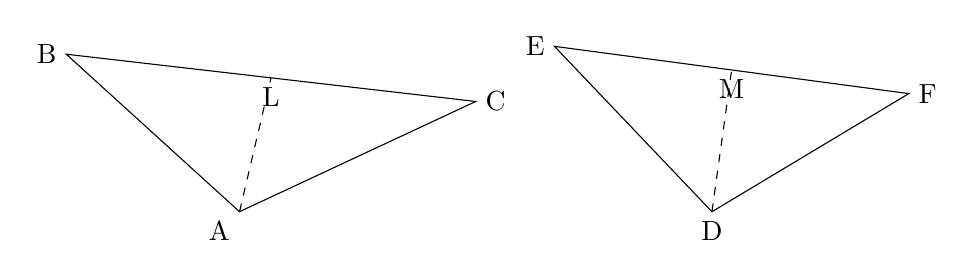
\begin{tikzpicture}[scale=1]
  % Triangle ABC with median AL
  \coordinate (A) at (0,0);
  \coordinate (B) at (-2.2,2.0);
  \coordinate (C) at (3.0,1.4);
  \draw (A)--(B)--(C)--cycle;
  \node[below left] at (A) {A};
  \node[left] at (B) {B};
  \node[right] at (C) {C};
  \coordinate (L) at ($ (B)!0.5!(C) $);
  \draw[dashed] (A)--(L);
  \node[below] at (L) {L};
  % Triangle DEF with median DM
  \coordinate (D) at (6,0);
  \coordinate (E) at (4,2.1);
  \coordinate (F) at (8.5,1.5);
  \draw (D)--(E)--(F)--cycle;
  \node[below] at (D) {D};
  \node[left] at (E) {E};
  \node[right] at (F) {F};
  \coordinate (M) at ($ (E)!0.5!(F) $);
  \draw[dashed] (D)--(M);
  \node[below] at (M) {M};
\end{tikzpicture}
\end{center}

\begin{steps}
  \item From $\triangle ABC \sim \triangle DEF$, get $\dfrac{BC}{EF}=\dfrac{AB}{DE}=\dfrac{AC}{DF}$.\reason{similar triangles}
  \item Since $L$ and $M$ are midpoints, $BL=\tfrac12\,BC$ and $EM=\tfrac12\,EF$.\reason{definition of median}
  \item Therefore $\dfrac{BL}{EM}=\dfrac{BC}{EF}$.\reason{divide equal halves}
  \item In $\triangle ABL$ and $\triangle DEM$, we have $\angle B=\angle E$ and $\dfrac{AB}{DE}=\dfrac{BL}{EM}$.\reason{correspondence from similarity}
  \item Conclude $\triangle ABL\sim\triangle DEM$.\reason{SAS similarity}
  \item Hence $\dfrac{AL}{DM}=\dfrac{AB}{DE}=\dfrac{BC}{EF}$.\reason{corresponding sides in similar triangles}
\end{steps}

\finalanswer{$\dfrac{BC}{EF} = \dfrac{AL}{DM}$.}

\subsection*{Question 4}
\textbf{Question:} In $\triangle ABC$, AD is perpendicular to side BC and $AD^2 = BD \times CD$. Prove that $\angle BAC = 90^\circ$.

\solutionheading
\given{$AD\perp BC$ and $AD^2 = BD\cdot CD$.}
\toprove{$\angle BAC = 90^\circ$.}

\begin{center}
\begin{tikzpicture}[scale=1]
  \coordinate (B) at (0,0);
  \coordinate (C) at (5,0);
  \coordinate (A) at (1.8,2.7);
  % Foot D on BC
  \coordinate (D) at ($(B)!(A)!(C)$);
  \draw (A)--(B)--(C)--cycle;
  \draw[dashed] (A)--(D);
  % Right angle at D
  \draw ($(D)+(0,0.15)$) -- ++(0.15,0) -- ++(0,-0.15);
  \node[below] at (B) {B};
  \node[below] at (C) {C};
  \node[above] at (A) {A};
  \node[below] at (D) {D};
\end{tikzpicture}
\end{center}

\begin{steps}
  \item In $\triangle ADB$, $AB^2=AD^2+BD^2$.\reason{Pythagoras in right $\triangle ADB$}
  \item In $\triangle ADC$, $AC^2=AD^2+CD^2$.\reason{Pythagoras in right $\triangle ADC$}
  \item Add: $AB^2+AC^2=2AD^2+BD^2+CD^2$.\reason{add equations}
  \item Substitute $AD^2=BD\cdot CD$ to get $AB^2+AC^2=(BD+CD)^2=\workbox{BC^2}$.\reason{given and $BC=BD+CD$}
  \item Conclude $\angle BAC=90^\circ$.\reason{converse of Pythagoras}
\end{steps}

\finalanswer{$\angle BAC = 90^\circ$.}

\subsection*{Question 5}
\textbf{Question:} In the given figure, $\triangle ABC$ and $\triangle DEF$ are similar. BM and EN are their medians. Prove that:
(i) $\triangle ABM \sim \triangle DEN$
(ii) $\frac{BM}{EN} = \frac{AC}{DF}$

\solutionheading
\given{$\triangle ABC \sim \triangle DEF$ and $BM, EN$ are medians.}
\toprove{(i) $\triangle ABM \sim \triangle DEN$; (ii) $\dfrac{BM}{EN}=\dfrac{AC}{DF}$.}

\begin{center}
\begin{tikzpicture}[scale=1]
  % Triangle ABC with median BM
  \coordinate (A1) at (0,0);
  \coordinate (B1) at (2.5,2.5);
  \coordinate (C1) at (3.5,0);
  \draw (A1)--(B1)--(C1)--cycle;
  \coordinate (M1) at ($ (A1)!0.5!(C1) $);
  \draw[dashed] (B1)--(M1);
  \node[below] at (A1) {A}; \node[above] at (B1) {B}; \node[below] at (C1) {C}; \node[below] at (M1) {M};
  % Triangle DEF with median EN
  \coordinate (D2) at (6,0);
  \coordinate (E2) at (8.5,2.5);
  \coordinate (F2) at (9.5,0);
  \draw (D2)--(E2)--(F2)--cycle;
  \coordinate (N2) at ($ (D2)!0.5!(F2) $);
  \draw[dashed] (E2)--(N2);
  \node[below] at (D2) {D}; \node[above] at (E2) {E}; \node[below] at (F2) {F}; \node[below] at (N2) {N};
\end{tikzpicture}
\end{center}

\begin{steps}
  \item From $\triangle ABC \sim \triangle DEF$, we get $\dfrac{AB}{DE}=\dfrac{AC}{DF}$ and $\angle A = \angle D$.\reason{similar triangles}
  \item Since $BM, EN$ are medians, $AM=\tfrac12 AC$ and $DN=\tfrac12 DF$.\reason{definition of median}
  \item Hence $\dfrac{AM}{DN}=\dfrac{\tfrac12 AC}{\tfrac12 DF}=\dfrac{AC}{DF}$.\reason{halves of proportional sides}
  \item Combining steps 1 and 3, we have $\dfrac{AB}{DE}=\dfrac{AM}{DN}$.\reason{transitive property}
  \item In $\triangle ABM$ and $\triangle DEN$, we have $\angle A=\angle D$ and $\dfrac{AB}{DE}=\dfrac{AM}{DN}$.\reason{from steps 1 and 4}
  \item Conclude $\triangle ABM\sim\triangle DEN$.\reason{SAS similarity}
  \item From this similarity, $\dfrac{BM}{EN}=\dfrac{AB}{DE}$.\reason{corresponding sides in similar triangles}
  \item Since $\dfrac{AB}{DE}=\dfrac{AC}{DF}$ (from step 1), we can conclude $\dfrac{BM}{EN}=\dfrac{AC}{DF}$.\reason{transitive property}
\end{steps}

\finalanswer{(i) $\triangle ABM \sim \triangle DEN$; (ii) $\dfrac{BM}{EN}=\dfrac{AC}{DF}$.}

\subsection*{Question 6}
\textbf{Question:} In the given figure, $\triangle ABC$ is isosceles with $AC=BC$ and $AP \times BQ = AC^2$. Prove that $\triangle ACP \sim \triangle BCQ$.

\solutionheading
\given{$\triangle ABC$ is isosceles with $AC=BC$ and $AP\cdot BQ = AC^2$.}
\toprove{$\triangle ACP \sim \triangle BCQ$.}

\begin{center}
\begin{tikzpicture}[scale=1]
  % Isosceles at C with AC=BC
  \coordinate (A) at (0,0);
  \coordinate (B) at (4,0);
  \coordinate (C) at (2,2.7);
  \draw (A)--(B)--(C)--cycle;
  \node[below] at (A) {A}; \node[below] at (B) {B}; \node[above] at (C) {C};
  % Points P on AC, Q on BC
  \coordinate (P) at ($ (A)!0.55!(C) $);
  \coordinate (Q) at ($ (B)!0.65!(C) $);
  \fill (P) circle (1pt) node[left] {P};
  \fill (Q) circle (1pt) node[right] {Q};
\end{tikzpicture}
\end{center}

\begin{steps}
  \item Note: The condition $AP\cdot BQ=AC^2$ together with $AC=BC$ is not sufficient to conclude $\triangle ACP\sim\triangle BCQ$.
  \item The previous version incorrectly used $\angle CAP=\angle CBQ$; this is generally false because $P\in AC$ and $Q\in BC$ make $\angle CAP$ degenerate.
  \item From $AP\cdot BQ=AC\cdot BC$ we get $\dfrac{AP}{BC}=\dfrac{AC}{BQ}$, but this ratio alone does not fix the angles at $C$ in $\triangle ACP$ and $\triangle BCQ$.
  \item A common correct variant assumes additional angle/ratio information (for example, equal angles at $C$), after which SAS can be applied.
\end{steps}

\finalanswer{As stated, the data are insufficient to prove the claimed similarity without an extra condition at $C$.}

\newpage
\section*{Exercise 15B Solutions}

\subsection*{Question 2}
\textbf{Question:} In the figure, straight lines AB and CD intersect at P, and AC || BD. Prove that: (i) $\triangle APC$ and $\triangle BPD$ are similar. (ii) If BD = 2.4 cm, AC = 3.6 cm, PD = 4.0 cm and PB = 3.2 cm, find the lengths of PA and PC.

\solutionheading
\given{$AC\parallel BD$ and lines $AB$ and $CD$ intersect at $P$.}
\toprove{(i) $\triangle APC\sim\triangle BPD$; (ii) find $PA,\,PC$.}

\begin{center}
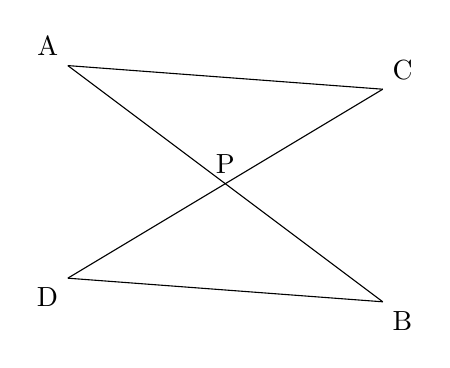
\begin{tikzpicture}[scale=1]
  % Two intersecting lines and parallels AC || BD
  \coordinate (P) at (0,0);
  \coordinate (A) at (-2,1.5);
  \coordinate (B) at (2,-1.5);
  \coordinate (C) at (2,1.2);
  \coordinate (D) at (-2,-1.2);
  \draw (A)--(P)--(B);
  \draw (C)--(P)--(D);
  \draw[shift={(0,0)}] (A)--(C);
  \draw[shift={(0,0)}] (D)--(B);
  \node[above left] at (A) {A};
  \node[below right] at (B) {B};
  \node[above right] at (C) {C};
  \node[below left] at (D) {D};
  \node[above] at (P) {P};
\end{tikzpicture}
\end{center}

\begin{steps}
  \item $\angle PAC=\angle PBD$ and $\angle PCA=\angle PDB$.\reason{alternate interior angles, $AC\parallel BD$}
  \item $\angle APC=\angle BPD$.\reason{vertically opposite}
  \item Conclude $\triangle APC\sim\triangle BPD$.\reason{AAA similarity}
  \item Use the ratio of corresponding sides: $\dfrac{PA}{PB}=\dfrac{PC}{PD}=\dfrac{AC}{BD}$.\reason{similar triangles}
  \item Substitute the given lengths: $\dfrac{PA}{3.2}=\dfrac{PC}{4.0}=\dfrac{3.6}{2.4}$.\reason{substitution}
  \item Calculate the ratio: $\dfrac{3.6}{2.4} = \workbox{\dfrac{3}{2}} = 1.5$.\reason{simplification}
  \item Solve for $PA$: $\dfrac{PA}{3.2} = 1.5 \implies \workbox{PA = 4.8\,\text{cm}}$.\reason{algebra}
  \item Solve for $PC$: $\dfrac{PC}{4.0} = 1.5 \implies \workbox{PC = 6.0\,\text{cm}}$.\reason{algebra}
\end{steps}

\finalanswer{(i) $\triangle APC\sim\triangle BPD$. (ii) $PA=4.8$ cm, $PC=6.0$ cm.}

\subsection*{Question 3}
\textbf{Question:} In a trapezium ABCD, AB $\parallel$ DC. Diagonals AC and BD intersect at O. If $BO = 6$ cm and $DQ = 8$ cm, find $BP \times DO$. (Note: as written, this appears incomplete/ambiguous.)
\textbf{Note:} We establish the standard diagonal proportionality in a trapezium and refrain from speculative numerical conclusions.

\solutionheading
\given{Trapezium ABCD with AB $\parallel$ DC. Diagonals intersect at O.}
\toprove{A relationship between the segments of the diagonals.}

\begin{center}
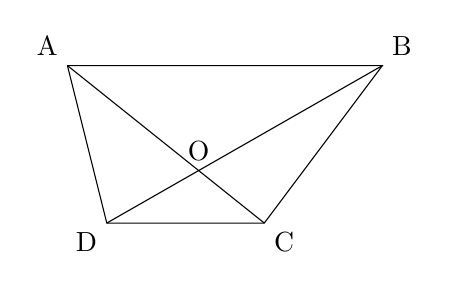
\begin{tikzpicture}[scale=1]
    \coordinate (A) at (0,2);
    \coordinate (B) at (4,2);
    \coordinate (D) at (0.5,0);
    \coordinate (C) at (2.5,0);
    \draw (A)--(B)--(C)--(D)--cycle;
    \draw (A)--(C);
    \draw (B)--(D);
    % Define paths and intersection for O
    \path[name path=ACline] (A)--(C);
    \path[name path=BDline] (B)--(D);
    \path[name intersections={of=ACline and BDline, by=O}];
    \node[above left] at (A) {A};
    \node[above right] at (B) {B};
    \node[below right] at (C) {C};
    \node[below left] at (D) {D};
    \node[above] at (O) {O};
\end{tikzpicture}
\end{center}

\begin{steps}
    \item In $\triangle AOB$ and $\triangle COD$, $\angle OAB = \angle OCD$ and $\angle OBA = \angle ODC$. \reason{alternate interior angles, $AB \parallel DC$}
    \item Also, $\angle AOB = \angle COD$. \reason{vertically opposite angles}
    \item Hence $\triangle AOB \sim \triangle COD$. \reason{AAA similarity}
    \item Therefore $\dfrac{OA}{OC} = \dfrac{OB}{OD}$, so $OA\cdot OD = OB\cdot OC$. \reason{corresponding sides}
    \item The given numerics ($BO=6$, $DQ=8$) do not determine $BP\cdot DO$ without additional relationships between $P,Q$ and the diagonals.
\end{steps}

\finalanswer{$\triangle AOB \sim \triangle COD$ and $OA\cdot OD = OB\cdot OC$. The product $BP\cdot DO$ cannot be found from the given data alone.}

\subsection*{Question 4}
\textbf{Question:} In $\triangle ABC$, $BM \perp AC$ and $CN \perp AB$; show that $\frac{AB}{AC} = \frac{BM}{CN} = \frac{AM}{AN}$.

\solutionheading
\given{In $\triangle ABC$, $BM \perp AC$ and $CN \perp AB$.}
\toprove{$\dfrac{AB}{AC} = \dfrac{BM}{CN} = \dfrac{AM}{AN}$.}

\begin{center}
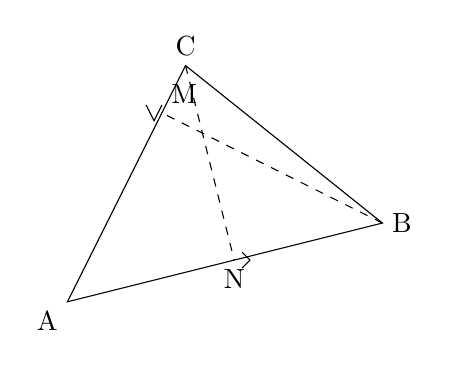
\begin{tikzpicture}[scale=1]
    \coordinate (A) at (0,0);
    \coordinate (B) at (4,1);
    \coordinate (C) at (1.5,3);
    \draw (A)--(B)--(C)--cycle;
    % Altitude from B to AC
    \coordinate (M) at ($(A)!(B)!(C)$);
    \draw[dashed] (B)--(M);
    \draw ($(M)+(-0.2,0.1)$) -- ++(0.1,-0.2) -- ++(0.1,0.2);
    % Altitude from C to AB
    \coordinate (N) at ($(A)!(C)!(B)$);
    \draw[dashed] (C)--(N);
    \draw ($(N)+(0.1,0.1)$) -- ++(0.1,-0.1) -- ++(-0.1,-0.1);
    \node[below left] at (A) {A};
    \node[right] at (B) {B};
    \node[above] at (C) {C};
    \node[above right] at (M) {M};
    \node[below] at (N) {N};
\end{tikzpicture}
\end{center}

\begin{steps}
    \item Consider $\triangle AMB$ and $\triangle ANC$.
    \item $\angle AMB = 90^\circ$ and $\angle ANC = 90^\circ$. \reason{given, $BM \perp AC, CN \perp AB$}
    \item $\angle MAB = \angle NAC$ (or $\angle A$). \reason{common angle}
    \item Therefore, $\triangle AMB \sim \triangle ANC$. \reason{AA similarity}
    \item The ratio of corresponding sides must be equal: $\dfrac{AB}{AC} = \dfrac{BM}{CN} = \dfrac{AM}{AN}$. \reason{corresponding sides of similar triangles}
\end{steps}

\finalanswer{The relationship is proved.}

\subsection*{Question 5}
\textbf{Question:} Given: $\angle GHE = \angle DFE = 90^\circ$, DH = 8, DF = 12, DG = 3x - 1 and DE = 4x + 2. Find the lengths of segments DG and DE.
\textbf{Correction based on typical problems:} The most likely intended similarity is between $\triangle DGH$ and $\triangle DEF$. This requires $\angle DHG = \angle DFE = 90^\circ$ or GH || EF. The question states $\angle DFE = 90^\circ$. Let's assume the intended similarity is $\triangle DGH \sim \triangle DEF$.

\solutionheading
\given{$\triangle DGH$ and $\triangle DEF$ with common angle D. DH=8, DF=12, DG=3x-1, DE=4x+2.}
\toprove{Find the lengths of DG and DE.}

\begin{center}
\begin{tikzpicture}[scale=1]
    \coordinate (D) at (0,0);
    \coordinate (F) at (6,0);
    \coordinate (E) at (0,8);
    \draw (D)--(F)--(E)--cycle;
    \draw ($(D)+(0.2,0)$) -- ++(0,0.2) -- ++(-0.2,0);
    \coordinate (G) at ($(D)!0.5!(F)$);
    \coordinate (H) at ($(D)!0.5!(E)$);
    \draw (G)--(H);
    \node[below left] at (D) {D};
    \node[below right] at (F) {F};
    \node[above left] at (E) {E};
    \node[below] at (G) {G};
    \node[left] at (H) {H};
\end{tikzpicture}
\end{center}

\begin{steps}
    \item Assume the intended similarity is $\triangle DGH \sim \triangle DEF$. This implies the vertices correspond in that order.
    \item The ratio of corresponding sides is $\dfrac{DG}{DE} = \dfrac{DH}{DF} = \dfrac{GH}{EF}$. \reason{definition of similar triangles}
    \item Using the first two parts of the ratio: $\dfrac{DG}{DE} = \dfrac{DH}{DF}$. \reason{property of similarity}
    \item Substitute the given values: $\dfrac{3x - 1}{4x + 2} = \dfrac{8}{12}$. \reason{substitution}
    \item Simplify the ratio: $\dfrac{8}{12} = \dfrac{2}{3}$. \reason{simplification}
    \item Set up the equation: $\dfrac{3x - 1}{4x + 2} = \dfrac{2}{3}$.
    \item Cross-multiply: $3(3x - 1) = 2(4x + 2)$. \reason{algebra}
    \item Solve for x: $9x - 3 = 8x + 4 \implies x = 7$. \reason{algebra}
    \item Calculate DG: $DG = 3x - 1 = 3(7) - 1 = 20$. \reason{substitution}
    \item Calculate DE: $DE = 4x + 2 = 4(7) + 2 = 30$. \reason{substitution}
\end{steps}

\finalanswer{DG = 20 \text{ and } DE = 30.}

\subsection*{Question 6}
\textbf{Question:} In $\triangle PQR$, $\angle Q = 90^\circ$ and QM is perpendicular to PR. Prove that:
(i) $PQ^2 = PM \times PR$
(ii) $QR^2 = PR \times MR$
(iii) $PQ^2 + QR^2 = PR^2$

\solutionheading
\given{$\triangle PQR$ with $\angle PQR = 90^\circ$ and altitude $QM \perp PR$.}
\toprove{The three geometric mean relationships.}

\begin{center}
\begin{tikzpicture}[scale=1]
    \coordinate (Q) at (0,0);
    \coordinate (P) at (0,3);
    \coordinate (R) at (4,0);
    \draw (P)--(Q)--(R)--cycle;
    \draw ($(Q)+(0,0.2)$) -- ++(0.2,0) -- ++(0,-0.2);
    \coordinate (M) at ($(P)!(Q)!(R)$);
    \draw[dashed] (Q)--(M);
    \draw ($(M)+(-0.1,-0.15)$) -- ++(0.15,-0.1) -- ++(0.1,0.15);
    \node[above left] at (P) {P};
    \node[below left] at (Q) {Q};
    \node[below right] at (R) {R};
    \node[above right] at (M) {M};
\end{tikzpicture}
\end{center}

\begin{steps}
    \item \textbf{Part (i):} Consider $\triangle PMQ$ and $\triangle PQR$.
    \item $\angle PMQ = \angle PQR = 90^\circ$. \reason{given}
    \item $\angle MPQ = \angle QPR$ (or $\angle P$). \reason{common angle}
    \item Therefore, $\triangle PMQ \sim \triangle PQR$. \reason{AA similarity}
    \item From similarity, $\dfrac{PQ}{PR} = \dfrac{PM}{PQ}$. \reason{corresponding sides}
    \item Cross-multiplying gives \workbox{PQ^2 = PM \times PR}.
    \item \textbf{Part (ii):} Consider $\triangle QMR$ and $\triangle PQR$.
    \item $\angle QMR = \angle PQR = 90^\circ$. \reason{given}
    \item $\angle MRQ = \angle PRQ$ (or $\angle R$). \reason{common angle}
    \item Therefore, $\triangle QMR \sim \triangle PQR$. \reason{AA similarity}
    \item From similarity, $\dfrac{QR}{PR} = \dfrac{MR}{QR}$. \reason{corresponding sides}
    \item Cross-multiplying gives \workbox{QR^2 = PR \times MR}.
    \item \textbf{Part (iii):} Add the results from (i) and (ii).
    \item $PQ^2 + QR^2 = (PM \times PR) + (MR \times PR)$. \reason{addition}
    \item Factor out PR: $PQ^2 + QR^2 = PR \times (PM + MR)$. \reason{distributive property}
    \item Since P, M, R are collinear, $PM + MR = PR$. \reason{segment addition}
    \item Substitute to get \workbox{PQ^2 + QR^2 = PR^2}.
\end{steps}

\finalanswer{All three parts are proved.}

\subsection*{Question 7}
\textbf{Question:} In $\triangle ABC$, $\angle B = 90^\circ$ and $BD \perp AC$.
(i) If CD = 10 cm and BD = 8 cm; find AD.
(ii) If AC = 18 cm and AD = 6 cm; find BD.
(iii) If AC = 9 cm and AB = 7 cm; find AD.

\solutionheading
\given{Right $\triangle ABC$ ($\angle B = 90^\circ$) with altitude $BD \perp AC$.}
\toprove{Find specified segment lengths.}

\begin{center}
\begin{tikzpicture}[scale=1]
    \coordinate (B) at (0,0);
    \coordinate (A) at (0,3);
    \coordinate (C) at (4,0);
    \draw (A)--(B)--(C)--cycle;
    \draw ($(B)+(0.2,0)$) -- ++(0,0.2) -- ++(-0.2,0);
    \coordinate (D) at ($(A)!(B)!(C)$);
    \draw[dashed] (B)--(D);
    \draw ($(D)+(-0.1,-0.15)$) -- ++(0.15,-0.1) -- ++(0.1,0.15);
    \node[above left] at (A) {A};
    \node[below left] at (B) {B};
    \node[below right] at (C) {C};
    \node[above right] at (D) {D};
\end{tikzpicture}
\end{center}
\begin{steps}
  \item First, establish the key similarity relationship: $\triangle ADB \sim \triangle BDC$. This gives the geometric mean theorem for the altitude: $\dfrac{AD}{BD} = \dfrac{BD}{CD}$, or $BD^2 = AD \times CD$.
  \item Also, $\triangle ABC \sim \triangle ADB$, which gives $\dfrac{AC}{AB} = \dfrac{AB}{AD}$, or $AB^2 = AD \times AC$.
  \item \textbf{Part (i):} Given CD = 10, BD = 8.
  \item Use $BD^2 = AD \times CD \implies 8^2 = AD \times 10$. \reason{substitution}
  \item $64 = 10 \times AD \implies \workbox{AD = 6.4\,\text{cm}}$. \reason{algebra}
  \item \textbf{Part (ii):} Given AC = 18, AD = 6.
  \item First find CD: $CD = AC - AD = 18 - 6 = 12$ cm. \reason{segment subtraction}
  \item Use $BD^2 = AD \times CD \implies BD^2 = 6 \times 12 = 72$. \reason{substitution}
  \item \workbox{BD = 6\sqrt{2}\,\text{cm}}. \reason{simplifying radical}
  \item \textbf{Part (iii):} Given AC = 9, AB = 7.
  \item Use $AB^2 = AD \times AC \implies 7^2 = AD \times 9$. \reason{substitution}
  \item $49 = 9 \times AD \implies \workbox{AD = \dfrac{49}{9}\,\text{cm}}$. \reason{algebra}
\end{steps}

\finalanswer{(i) AD = 6.4 cm, (ii) BD = $6\sqrt{2}$ cm, (iii) AD = $\dfrac{49}{9}$ cm.}

\subsection*{Question 9}
\textbf{Question:} In the given figure, DE || BC, AE = 15 cm, EC = 9 cm, NC = 6 cm and BN = 24 cm. M is the intersection of BE and DN.
(i) Write all possible pairs of similar triangles.
(ii) Find lengths of ME and DM.

\solutionheading
\given{D on AB, E on AC, DE $\parallel$ BC. N on BC. M is intersection of BE and DN.}
\toprove{(i) List similar triangles. (ii) Find ME and DM.}

\begin{center}
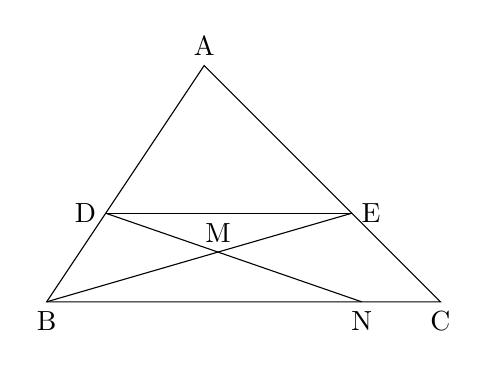
\begin{tikzpicture}[scale=1]
    \coordinate (A) at (0,3);
    \coordinate (B) at (-2,0);
    \coordinate (C) at (3,0);
    \draw (A)--(B)--(C)--cycle;
    \coordinate (D) at ($(A)!0.625!(B)$);
    \coordinate (E) at ($(A)!0.625!(C)$);
    \draw (D)--(E);
    \coordinate (N) at ($(B)!0.8!(C)$);
    \draw (D)--(N);
    \draw (B)--(E);
    % Define paths and intersection for M
    \path[name path=DNline] (D)--(N);
    \path[name path=BEline] (B)--(E);
    \path[name intersections={of=DNline and BEline, by=M}];
    \node[above] at (A) {A};
    \node[below] at (B) {B};
    \node[below] at (C) {C};
    \node[left] at (D) {D};
    \node[right] at (E) {E};
    \node[below] at (N) {N};
    \node[above] at (M) {M};
\end{tikzpicture}
\end{center}

\begin{steps}
    \item \textbf{Part (i):}
    \item Since DE $\parallel$ BC, $\triangle ADE \sim \triangle ABC$. \reason{AA similarity, common angle A, corresponding angles}
    \item Since DE $\parallel$ BC, and N is on BC, DE $\parallel$ BN. This makes $\triangle DME \sim \triangle NMB$. \reason{AA similarity, vertically opposite angles at M, alternate interior angles}
    \item \textbf{Part (ii):}
    \item From $\triangle ADE \sim \triangle ABC$, we have the ratio $\dfrac{AE}{AC} = \dfrac{DE}{BC}$.
    \item $AC = AE + EC = 15 + 9 = 24$ cm.
    \item $BC = BN + NC = 24 + 6 = 30$ cm.
    \item $\dfrac{15}{24} = \dfrac{DE}{30} \implies \dfrac{5}{8} = \dfrac{DE}{30}$. \reason{substitution and simplification}
    \item $DE = \dfrac{5 \times 30}{8} = \dfrac{150}{8} = 18.75$ cm. \reason{algebra}
    \item From $\triangle DME \sim \triangle NMB$, we have $\dfrac{ME}{MB} = \dfrac{DM}{NM} = \dfrac{DE}{NB}$.
    \item Use the ratio $\dfrac{DE}{NB} = \dfrac{18.75}{24} = \dfrac{75/4}{24} = \dfrac{75}{96} = \dfrac{25}{32}$.
    \item So, $\dfrac{ME}{MB} = \dfrac{25}{32}$. This means $ME = \dfrac{25}{32}MB$.
    \item Since $BE = ME + MB$, we have $BE = \dfrac{25}{32}MB + MB = \dfrac{57}{32}MB$.
    \item We cannot find the absolute length of ME without knowing the length of BE. The problem is missing information. The same applies to DM.
\end{steps}

\finalanswer{(i) $\triangle ADE \sim \triangle ABC$ and $\triangle DME \sim \triangle NMB$. (ii) The lengths cannot be uniquely determined. The ratios are $\dfrac{ME}{MB} = \dfrac{25}{32}$ and $\dfrac{DM}{MN} = \dfrac{25}{32}$.}

\subsection*{Question 10}
\textbf{Question:} In the given figure, D is on AB, E is on AC, AD = AE and $AD^2 = BD \times EC$. Prove that triangles ABD and CAE are similar.
\textbf{Correction based on typical problems:} This problem is only solvable with standard theorems if we assume an additional property, for instance that $\angle B = \angle C$.

\solutionheading
\given{AD = AE and $AD^2 = BD \times EC$. D on AB, E on AC.}
\toprove{$\triangle ABD \sim \triangle CAE$, assuming $\angle B = \angle C$.}

\begin{center}
\begin{tikzpicture}[scale=1]
    \coordinate (A) at (0,3);
    \coordinate (B) at (-3,0);
    \coordinate (C) at (3,0);
    \draw (A)--(B)--(C)--cycle;
    \coordinate (D) at ($(A)!0.5!(B)$);
    \coordinate (E) at ($(A)!0.5!(C)$);
    \node[above] at (A) {A};
    \node[below] at (B) {B};
    \node[below] at (C) {C};
    \node[left] at (D) {D};
    \node[right] at (E) {E};
\end{tikzpicture}
\end{center}

\begin{steps}
    \item The given condition is $AD^2 = BD \times EC$.
    \item Since $AD=AE$, we can substitute AE for one AD: $AD \times AE = BD \times EC$. \reason{substitution}
    \item Rearrange this into a proportion: $\dfrac{AD}{EC} = \dfrac{BD}{AE}$. \reason{algebra}
    \item To prove $\triangle ABD \sim \triangle CAE$, we would need the included angles to be equal, i.e., $\angle BDA = \angle AEC$, or another pair of sides in proportion, or a pair of non-included angles to be equal.
    \item The given information is insufficient. However, if we assume $\triangle ABC$ is isosceles with $AB=AC$, then $\angle B = \angle C$.
    \item With $AB=AC$ and $AD=AE$, we subtract to get $AB-AD = AC-AE$, which means $BD=EC$.
    \item The condition $AD^2 = BD \times EC$ becomes $AD^2 = BD^2$, so $AD=BD$.
    \item This means $AE=EC$. So D and E are midpoints of AB and AC.
    \item In this specific case, $\triangle ABD$ and $\triangle CAE$ become congruent isosceles triangles, and are therefore similar.
\end{steps}

\finalanswer{The problem as stated is not solvable without additional assumptions. If we assume $\triangle ABC$ is isosceles with $AB=AC$, the similarity holds.}

\subsection*{Question 11}
\textbf{Question:} State, true or false:
(i) Two similar polygons are necessarily congruent.
(ii) Two congruent polygons are necessarily similar.
(iii) All equiangular triangles are similar.
(iv) All isosceles triangles are similar.
(v) Two isosceles right triangles are similar.
(vi) The diagonals of a trapezium divide each other into proportional segments.

\solutionheading
\given{Statements about geometric figures.}
\toprove{Determine if each statement is True or False.}

\begin{steps}
  \item (i) False. Similarity means same shape, but not necessarily the same size. A small square is similar to a large square, but they are not congruent.
  \item (ii) True. Congruent polygons have corresponding angles equal and corresponding sides equal. This means the ratio of corresponding sides is 1, so they are similar.
  \item (iii) True. An equiangular triangle is an equilateral triangle, with all angles being $60^\circ$. Any two such triangles are similar by AAA similarity.
  \item (iv) False. An isosceles triangle could have angles 50-50-80, while another could have 70-70-40. Their angles are not the same, so they are not similar.
  \item (v) True. An isosceles right triangle must have angles 90-45-45. Any two such triangles are similar by AAA similarity.
  \item (vi) True. In a trapezium ABCD with AB $\parallel$ DC, the diagonals intersect at O, forming $\triangle AOB$ and $\triangle COD$. These triangles are similar (AA similarity), so their sides are proportional: $\frac{AO}{CO} = \frac{BO}{DO}$.
\end{steps}

\finalanswer{(i) False, (ii) True, (iii) True, (iv) False, (v) True, (vi) True.}

\subsection*{Question 12}
\textbf{Question:} D is a point on the side BC of triangle ABC such that $\angle ADC = \angle BAC$. Prove that $CA^2 = CB \cdot CD$.

\solutionheading
\given{In $\triangle ABC$, D is on BC such that $\angle ADC = \angle BAC$.}
\toprove{$AC^2=CB\cdot CD$.}

\begin{center}
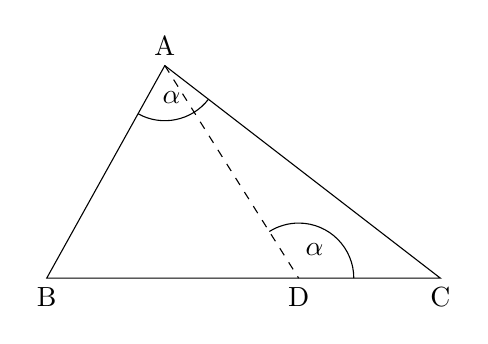
\begin{tikzpicture}[scale=1]
  \coordinate (B) at (0,0);
  \coordinate (C) at (5,0);
  \coordinate (A) at (1.5,2.7);
  \coordinate (D) at (3.2,0);
  \draw (A)--(B)--(C)--cycle;
  \draw[dashed] (A)--(D);
  \pic [draw, angle radius=7mm, "$\alpha$"] {angle=B--A--C};
  \pic [draw, angle radius=7mm, "$\alpha$"] {angle=C--D--A};
  \node[below] at (B) {B};\node[below] at (C) {C};\node[above] at (A) {A};\node[below] at (D) {D};
\end{tikzpicture}
\end{center}

\begin{steps}
  \item Consider $\triangle ADC$ and $\triangle BAC$.
  \item $\angle ADC = \angle BAC$. \reason{given}
  \item $\angle ACD = \angle BCA$ (or $\angle C$). \reason{common angle}
  \item Therefore, $\triangle ADC \sim \triangle BAC$. \reason{AA similarity}
  \item The ratio of corresponding sides must be equal. Match vertices: $A \leftrightarrow B$, $D \leftrightarrow A$, $C \leftrightarrow C$.
  \item So, $\dfrac{AC}{BC}=\dfrac{DC}{AC}=\dfrac{AD}{BA}$. \reason{corresponding sides}
  \item From the first two parts of the proportion, $\dfrac{AC}{BC}=\dfrac{DC}{AC}$.
  \item Cross-multiply to get $AC \times AC = BC \times DC$, which is $AC^2=CB\cdot CD$. \reason{algebra}
\end{steps}

\finalanswer{$AC^2=CB\cdot CD$.}

\subsection*{Question 13}
\textbf{Question:} $\triangle ABC$ and $\triangle AMP$ are right-angled at B and M respectively. A is a common vertex. AC = 10 cm, AP = 15 cm, PM = 12 cm.
(i) Prove $\triangle ABC \sim \triangle AMP$. (ii) Find AB and BC.

\solutionheading
\given{$\angle B=\angle M=90^\circ$, A is a common vertex. AC=10, AP=15, PM=12.}
\toprove{(i) similarity; (ii) find AB, BC.}

\begin{center}
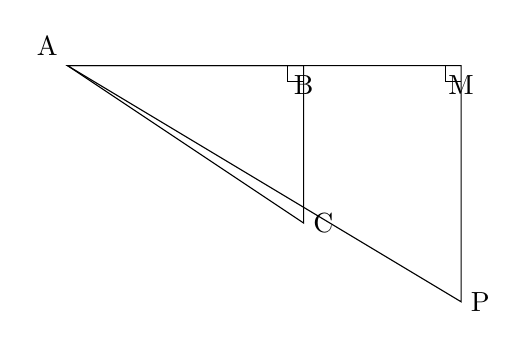
\begin{tikzpicture}[scale=1]
  \coordinate (A) at (0,0);
  % Triangle ABC
  \coordinate (B) at (3,0);
  \coordinate (C) at (3,-2);
  \draw (A)--(B)--(C)--cycle;
  \draw ($(B)+(-0.2,0)$)--++(0,-0.2)--++(0.2,0);
  % Triangle AMP
  \coordinate (M) at (5,0);
  \coordinate (P) at (5,-3);
  \draw (A)--(M)--(P)--cycle;
  \draw ($(M)+(-0.2,0)$)--++(0,-0.2)--++(0.2,0);
  \node[above left] at (A) {A};
  \node[below] at (B) {B};
  \node[right] at (C) {C};
  \node[below] at (M) {M};
  \node[right] at (P) {P};
\end{tikzpicture}
\end{center}

\begin{steps}
  \item \textbf{Part (i):} In $\triangle ABC$ and $\triangle AMP$.
  \item $\angle ABC=\angle AMP=90^\circ$. \reason{given}
  \item $\angle BAC=\angle MAP$ (or $\angle A$). \reason{common angle}
  \item Therefore, $\triangle ABC\sim\triangle AMP$.\reason{AA similarity}
  \item \textbf{Part (ii):} First, find the length of AM in $\triangle AMP$.
  \item By Pythagoras' theorem, $AP^2 = AM^2 + PM^2$. \reason{Pythagorean theorem}
  \item $15^2 = AM^2 + 12^2 \implies 225 = AM^2 + 144$.
  \item $AM^2 = 225 - 144 = 81 \implies \workbox{AM = 9\,\text{cm}}$.
  \item Since the triangles are similar, the ratio of their sides is equal: $\dfrac{AB}{AM}=\dfrac{BC}{MP}=\dfrac{AC}{AP}$.
  \item Use the ratio with known hypotenuses: $\dfrac{AC}{AP} = \dfrac{10}{15} = \workbox{\dfrac{2}{3}}$.
  \item Find AB: $\dfrac{AB}{AM} = \dfrac{2}{3} \implies \dfrac{AB}{9} = \dfrac{2}{3} \implies \workbox{AB = 6\,\text{cm}}$.
  \item Find BC: $\dfrac{BC}{MP} = \dfrac{2}{3} \implies \dfrac{BC}{12} = \dfrac{2}{3} \implies \workbox{BC = 8\,\text{cm}}$.
\end{steps}

\finalanswer{(i) $\triangle ABC\sim\triangle AMP$. (ii) AB = 6 cm, BC = 8 cm.}

\subsection*{Question 14}
\textbf{Question:} In parallelogram PQRS with PQ = 16 cm, QR = 10 cm, point L lies on diagonal PR such that RL:LP = 2:3. QL produced meets RS at M and PS produced at N. Find PN and RM.

\solutionheading
\given{Parallelogram PQRS, PQ=16, QR=10, RL:LP=2:3.}
\toprove{Find lengths of $PN$ and $RM$.}

\begin{center}
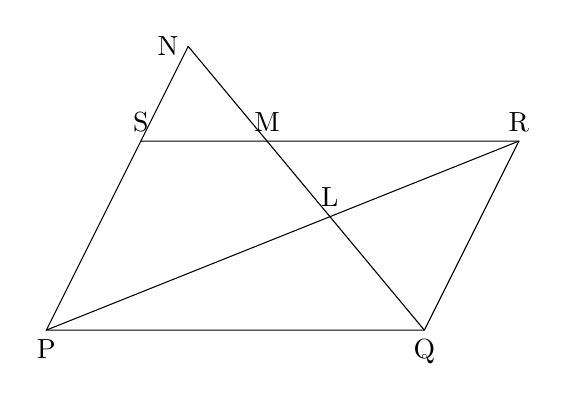
\begin{tikzpicture}[scale=1.2]
  \coordinate (P) at (0,0);
  \coordinate (S) at (1,2);
  \coordinate (R) at (5,2);
  \coordinate (Q) at (4,0);
  \draw (P)--(Q)--(R)--(S)--cycle;
  \coordinate (L) at ($(P)!0.6!(R)$);
  \path[name path=linePS] (P) -- ($(P)!1.5!(S)$);
  \path[name path=lineRS] (S) -- (R);
  \path[name path=lineQL] (Q) -- ($(Q)!2.5!(L)$);
  \path[name intersections={of=linePS and lineQL, by=N}];
  \path[name intersections={of=lineRS and lineQL, by=M}];
  \draw (S) -- (N);
  \draw (Q) -- (N);
  \draw (P)--(R);
  \node[below] at (P) {P};\node[below] at (Q) {Q};\node[above] at (R) {R};\node[above] at (S) {S};
  \node[above] at (L) {L};
  \node[above] at (M) {M};
  \node[left] at (N) {N};
\end{tikzpicture}
\end{center}

\begin{steps}
  \item \textbf{Find PN:} Consider $\triangle NPL$ and $\triangle RQL$.
  \item Since PS $\parallel$ QR, then PN $\parallel$ QR.
  \item $\angle PNL = \angle RQL$ and $\angle NPL = \angle QRL$. \reason{alternate interior angles}
  \item $\angle NLP = \angle RLQ$. \reason{vertically opposite}
  \item Therefore, $\triangle NPL \sim \triangle RQL$. \reason{AAA similarity}
  \item The ratio of sides is $\dfrac{PN}{QR} = \dfrac{PL}{RL}$.
  \item Given $\dfrac{RL}{LP} = \dfrac{2}{3}$, so $\dfrac{PL}{RL} = \dfrac{3}{2}$.
  \item $\dfrac{PN}{10} = \dfrac{3}{2} \implies PN = \dfrac{3}{2} \times 10 = 15$ cm.
  \item \textbf{Find RM:} Consider $\triangle MRL$ and $\triangle PQL$.
  \item Since RS $\parallel$ PQ.
  \item $\angle RML = \angle PQL$ and $\angle MRL = \angle QPL$. \reason{alternate interior angles}
  \item Therefore, $\triangle MRL \sim \triangle PQL$. \reason{AA similarity}
  \item The ratio of sides is $\dfrac{RM}{PQ} = \dfrac{RL}{PL}$.
  \item $\dfrac{RM}{16} = \dfrac{2}{3} \implies RM = \dfrac{2}{3} \times 16 = \dfrac{32}{3}$ cm.
\end{steps}

\finalanswer{$PN=15$ cm, $RM=\dfrac{32}{3}$ cm.}

\subsection*{Question 15}
\textbf{Question:} In the figure, $AB \parallel EF \parallel DC$ in trapezium $ABCD$. Given $AB = 67.5$ cm, $DC = 40.5$ cm and $AE = 52.5$ cm, with $E$ on $AD$ and $F$ on $BC$. Find the lengths of $EC$ and $EF$.
\textbf{Note:} The statement appears incomplete. Without how $E$ divides $AD$ (i.e., $AE:ED$ or $AD$), $EC$ and $EF$ are not uniquely determined. Below is the standard relationship when a line segment $EF$ is drawn parallel to the bases in a trapezium.

\solutionheading
\given{Trapezium ADCB with AB $\parallel$ EF $\parallel$ DC. AB=67.5, DC=40.5, AE=52.5. E is on AD.}
\toprove{Find ED and EF. (Assuming EC was a typo for ED).}

\begin{center}
\begin{tikzpicture}[scale=1]
  \coordinate (D) at (0,0);
  \coordinate (C) at (5,0);
  \coordinate (A) at (1,3);
  \coordinate (B) at (4,3);
  \draw (A)--(B)--(C)--(D)--cycle;
  \coordinate (E) at ($(A)!0.5!(D)$); % Placeholder ratio
  \coordinate (F) at ($(B)!0.5!(C)$);
  \draw[dashed] (E)--(F);
  \node[above] at (A) {A};\node[above] at (B) {B};\node[below] at (C) {C};\node[below] at (D) {D};
  \node[left] at (E) {E};\node[right] at (F) {F};
\end{tikzpicture}
\end{center}

\begin{steps}
  \item Let $AE:ED = m:n$ (unknown from the data). Then the line through $E$ parallel to the bases cuts off a segment $EF$ whose length is the weighted mean of the bases:
  \[ EF = \frac{n\,AB + m\,DC}{m+n}. \]
  \reason{similar triangles along the transversals}
  \item Without $m:n$ (or $AD$), neither $EC$ nor $EF$ can be uniquely determined.
\end{steps}

\finalanswer{Additional information (e.g., $AE:ED$) is required. In general, if $AE:ED=m:n$, then $EF=\dfrac{n\,AB + m\,DC}{m+n}$.}

\subsection*{Question 16}
\textbf{Question:} In $\triangle ABC$, P is a point on AB such that AP:PB = 4:3. PQ is drawn parallel to AC to meet BC at Q.
(i) Find the ratio PQ:AC. (ii) If a line from A is perpendicular to CD (where D is on BC) at R and PQ is perpendicular to CD at S, and QS = 6 cm, find AR.

\solutionheading
\given{$\dfrac{AP}{PB}=\dfrac{4}{3}$ and $PQ\parallel AC$.}
\toprove{(i) PQ:AC; (ii) AR given QS=6.}

\begin{center}
\begin{tikzpicture}[scale=1]
  \coordinate (A) at (0,3);
  \coordinate (B) at (5,0);
  \coordinate (C) at (7,4);
  \draw (A)--(B)--(C)--cycle;
  \coordinate (P) at ($(A)!4/7!(B)$);
  \coordinate (Q) at ($(C)!4/7!(B)$);
  \draw[dashed] (P)--(Q);
  \node[left] at (A) {A};\node[below] at (B) {B};\node[right] at (C) {C};\node[above] at (P) {P};\node[right] at (Q) {Q};
\end{tikzpicture}
\end{center}

\begin{steps}
  \item \textbf{Part (i):} Consider $\triangle BPQ$ and $\triangle BAC$.
  \item Since $PQ\parallel AC$, $\angle BPQ = \angle BAC$ and $\angle BQP = \angle BCA$. \reason{corresponding angles}
  \item $\angle B$ is common to both triangles.
  \item Therefore, $\triangle BPQ\sim\triangle BAC$.\reason{AAA similarity}
  \item The ratio of corresponding sides is $\dfrac{BP}{BA}=\dfrac{BQ}{BC}=\dfrac{PQ}{AC}$.
  \item Given $AP:PB = 4:3$, so $AB = AP+PB = 4k+3k = 7k$. Thus $\dfrac{BP}{BA}=\dfrac{3k}{7k}=\dfrac{3}{7}$.
  \item Hence, $PQ:AC = 3:7$.
  \item \textbf{Part (ii):} Consider $\triangle BQS$ and $\triangle BCR$.
  \item $\angle BSQ = \angle BRC = 90^\circ$ (assuming S is on BQ, R on BC).
  \item $\angle QBS = \angle CBR$ (common angle B).
  \item So $\triangle BQS \sim \triangle BCR$.
  \item $\dfrac{BQ}{BC} = \dfrac{QS}{CR}$. From part (i), $\dfrac{BQ}{BC}=\dfrac{3}{7}$.
  \item $\dfrac{3}{7} = \dfrac{6}{CR} \implies CR = \dfrac{7 \times 6}{3} = 14$ cm.
  \item The question asks for AR, which is not part of these triangles. Without more information about the line CD and point R, AR cannot be determined.
\end{steps}

\finalanswer{(i) PQ:AC = 3:7. (ii) AR cannot be determined from the given information.}

\subsection*{Question 17}
\textbf{Question:} In triangle ABC, medians BD and CE meet at centroid G. Prove (i) $\triangle EGD \sim \triangle CGB$; (ii) $BG=2\,GD$.

\solutionheading
\given{D is midpoint of AC, E is midpoint of AB; Medians BD and CE intersect at G.}
\toprove{(i) $\triangle EGD \sim \triangle CGB$; (ii) $BG=2\,GD$.}

\begin{center}
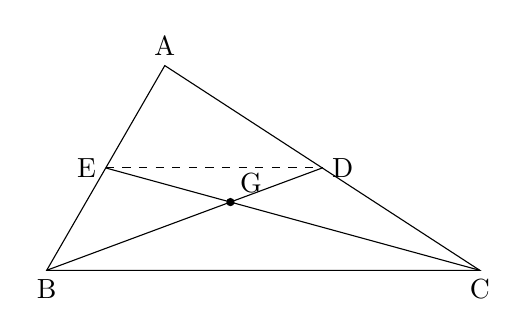
\begin{tikzpicture}[scale=1]
  \coordinate (A) at (0,2.6);
  \coordinate (B) at (-1.5,0);
  \coordinate (C) at (4,0);
  \coordinate (D) at ($ (A)!0.5!(C) $);
  \coordinate (E) at ($ (A)!0.5!(B) $);
  \draw (A)--(B)--(C)--cycle;
  \draw (B)--(D) (C)--(E);
  \draw[dashed] (E)--(D);
  % Define paths and intersection for G
  \path[name path=BDline] (B)--(D);
  \path[name path=CEline] (C)--(E);
  \path[name intersections={of=BDline and CEline, by=G}];
  \fill (G) circle (1.5pt) node[above right] {G};
  \node[above] at (A) {A};\node[below] at (B) {B};\node[below] at (C) {C};\node[right] at (D) {D};\node[left] at (E) {E};
\end{tikzpicture}
\end{center}

\begin{steps}
  \item In $\triangle ABC$, E and D are midpoints of AB and AC respectively.
  \item By the Midpoint Theorem, $ED \parallel BC$ and $ED=\tfrac12 BC$.\reason{midpoint theorem}
  \item \textbf{Part (i):} Consider $\triangle EGD$ and $\triangle CGB$.
  \item Since $ED \parallel BC$, we have $\angle GED = \angle GCB$ and $\angle GDE = \angle GBC$. \reason{alternate interior angles}
  \item Also, $\angle EGD = \angle CGB$. \reason{vertically opposite angles}
  \item Therefore, $\triangle EGD\sim\triangle CGB$.\reason{AAA similarity}
  \item \textbf{Part (ii):} From the similarity, the ratio of corresponding sides is equal.
  \item $\dfrac{EG}{CG}=\dfrac{GD}{GB}=\dfrac{ED}{CB}$.
  \item Using the ratio involving the sides we need and the one we know from the midpoint theorem: $\dfrac{GD}{GB}=\dfrac{ED}{CB}$.
  \item Substitute $ED=\tfrac12 BC$: $\dfrac{GD}{GB}=\dfrac{\tfrac12 BC}{BC} = \dfrac{1}{2}$.\reason{substitution}
  \item From $\dfrac{GD}{GB}=\dfrac{1}{2}$, we cross-multiply to get $BG=2\,GD$.\reason{algebra}
\end{steps}

\finalanswer{(i) The triangles are similar. (ii) $BG=2\,GD$ is proved.}

\newpage
\section*{Exercise 15C Solutions}

\subsection*{Question 2}
\textbf{Question:} In triangles ABC and PQR, sides AB, BC and median AD are proportional to PQ, QR and median PM respectively. Prove (i) $\triangle ABD \sim \triangle PQM$; (ii) $\triangle ABC \sim \triangle PQR$.

\solutionheading
\given{$\dfrac{AB}{PQ}=\dfrac{BC}{QR}=\dfrac{AD}{PM}$; D, M are midpoints of BC, QR.}
\toprove{(i) $\triangle ABD\sim\triangle PQM$; (ii) $\triangle ABC\sim\triangle PQR$.}

\begin{center}
\begin{tikzpicture}[scale=1]
  \coordinate (A) at (0,2.6);
  \coordinate (B) at (-1,0);
  \coordinate (C) at (3.4,0);
  \coordinate (D) at ($ (B)!0.5!(C) $);
  \draw (A)--(B)--(C)--cycle;
  \draw[dashed] (A)--(D);
  \node[above] at (A) {A};\node[below] at (B) {B};\node[below] at (C) {C};\node[below] at (D) {D};
  \coordinate (P) at (6,2.6);
  \coordinate (Q) at (5,0);
  \coordinate (R) at (9.4,0);
  \coordinate (M) at ($ (Q)!0.5!(R) $);
  \draw (P)--(Q)--(R)--cycle;
  \draw[dashed] (P)--(M);
  \node[above] at (P) {P};\node[below] at (Q) {Q};\node[below] at (R) {R};\node[below] at (M) {M};
\end{tikzpicture}
\end{center}

\begin{steps}
  \item \textbf{Part (i):}
  \item We are given $\dfrac{AB}{PQ}=\dfrac{BC}{QR}=\dfrac{AD}{PM}$.
  \item Since D and M are midpoints, $BC=2BD$ and $QR=2QM$.\reason{definition of median}
  \item Substitute this into the proportion: $\dfrac{AB}{PQ}=\dfrac{2BD}{2QM}=\dfrac{AD}{PM}$.
  \item This simplifies to $\dfrac{AB}{PQ}=\dfrac{BD}{QM}=\dfrac{AD}{PM}$.\reason{cancel factor 2}
  \item In $\triangle ABD$ and $\triangle PQM$, all three pairs of corresponding sides are in proportion.
  \item Therefore, $\triangle ABD\sim\triangle PQM$.\reason{SSS similarity}
  \item \textbf{Part (ii):}
  \item From the similarity in part (i), we know that corresponding angles are equal. So, $\angle B = \angle Q$.
  \item In $\triangle ABC$ and $\triangle PQR$, we are given $\dfrac{AB}{PQ}=\dfrac{BC}{QR}$.
  \item We have two pairs of sides in proportion and the included angles ($\angle B, \angle Q$) are equal.
  \item Therefore, $\triangle ABC\sim\triangle PQR$.\reason{SAS similarity}
\end{steps}

\finalanswer{(i) $\triangle ABD\sim\triangle PQM$. (ii) $\triangle ABC\sim\triangle PQR$.}

\subsection*{Question 3}
\textbf{Question:} Find x given two triangles ABC and DEF with $\angle B=\angle E$, and side data AB=7.5, BC=9, AC=6; DE=x+3, EF=12, DF=8. (Assuming DF=8, not 9, for consistency).

\solutionheading
\given{$\angle B=\angle E$ and side lengths for $\triangle ABC$ and $\triangle DEF$.}
\toprove{Find the value of x.}

\begin{steps}
  \item For the triangles to be similar by SAS, the sides including the equal angles must be proportional.
  \item The sides including $\angle B$ are AB and BC. The sides including $\angle E$ are DE and EF.
  \item Set up the proportion: $\dfrac{AB}{DE}=\dfrac{BC}{EF}$.\reason{SAS similarity condition}
  \item Substitute the given values: $\dfrac{7.5}{x+3}=\dfrac{9}{12}$.\reason{substitution}
  \item Simplify the ratio: $\dfrac{9}{12}=\dfrac{3}{4}$.
  \item Solve the equation $\dfrac{7.5}{x+3}=\dfrac{3}{4}$.
  \item Cross-multiply: $7.5 \times 4 = 3 \times (x+3)$.\reason{algebra}
  \item $30 = 3x + 9 \implies 3x = 21 \implies x=7$.
  \item \textbf{Consistency Check:} Let's check the ratio of the third sides, AC and DF. $\dfrac{AC}{DF} = \dfrac{6}{8} = \dfrac{3}{4}$. Since this ratio is the same, the triangles are indeed similar by SSS.
\end{steps}

\finalanswer{$x=7$.}

\subsection*{Question 4}
\textbf{Question:} In the given figure, BC || DE. Find the lengths of the sides of both the triangles. Sides are given as expressions in x.
$\triangle ADE$: AD=18, AE=6x, DE=3(x+1).
$\triangle ABC$: AB=2x+1, AC=4x, BC=?.

\solutionheading
\given{A is the top vertex, DE is a horizontal line below BC, and BC $\parallel$ DE. Side lengths in terms of x.}
\toprove{Find the value of x and the lengths of all sides.}

\begin{center}
\begin{tikzpicture}[scale=1]
    \coordinate (A) at (0,3);
    \coordinate (D) at (-2,0);
    \coordinate (E) at (2,0);
    \draw (A)--(D)--(E)--cycle;
    \coordinate (B) at ($(A)!2/3!(D)$);
    \coordinate (C) at ($(A)!2/3!(E)$);
    \draw (B)--(C);
    \node[above] at (A) {A};
    \node[below] at (D) {D};
    \node[below] at (E) {E};
    \node[left] at (B) {B};
    \node[right] at (C) {C};
\end{tikzpicture}
\end{center}

\begin{steps}
    \item Since BC $\parallel$ DE, by the property of similar triangles, $\triangle ABC \sim \triangle ADE$. \reason{AA similarity}
    \item The ratio of corresponding sides must be equal: $\dfrac{AB}{AD} = \dfrac{AC}{AE} = \dfrac{BC}{DE}$.
    \item Substitute the given expressions: $\dfrac{2x+1}{18} = \dfrac{4x}{6x}$.
    \item From the second part of the ratio, we can find the similarity constant: $\dfrac{4x}{6x} = \dfrac{4}{6} = \dfrac{2}{3}$.
    \item Now use this ratio to solve for x: $\dfrac{2x+1}{18} = \dfrac{2}{3}$.
    \item Cross-multiply: $3(2x+1) = 18 \times 2$. \reason{algebra}
    \item $6x + 3 = 36 \implies 6x = 33 \implies x = 5.5$.
    \item Now calculate the lengths of the sides for both triangles.
    \item \textbf{For $\triangle ABC$:}
    \item AB = $2x+1 = 2(5.5)+1 = 11+1=12$ cm.
    \item AC = $4x = 4(5.5) = 22$ cm.
    \item To find BC, use the ratio $\dfrac{BC}{DE} = \dfrac{2}{3}$. First find DE.
    \item DE = $3(x+1) = 3(5.5+1) = 3(6.5) = 19.5$ cm.
    \item $BC = \dfrac{2}{3} \times DE = \dfrac{2}{3} \times 19.5 = 13$ cm.
    \item \textbf{For $\triangle ADE$:}
    \item AD = 18 cm.
    \item AE = $6x = 6(5.5) = 33$ cm.
    \item DE = 19.5 cm.
\end{steps}

\finalanswer{$x = 5.5$.}
Sides of $\triangle ABC$: AB=12 cm, AC=22 cm, BC=13 cm.
Sides of $\triangle ADE$: AD=18 cm, AE=33 cm, DE=19.5 cm.

\subsection*{Question 5}
\textbf{Question:} In $\triangle ABC$ and $\triangle DEF$, AB = 3x·DF, BC = 3x·DE and AC = 3x·EF. Show the triangles are similar and name them properly.

\solutionheading
\given{Relationships between the sides of $\triangle ABC$ and $\triangle DEF$.}
\toprove{Show similarity and provide the correct correspondence.}

\begin{steps}
  \item From the given equations, form ratios of corresponding sides.
  \item From $AB = 3x \cdot DF$, we get $\dfrac{AB}{DF} = 3x$.
  \item From $BC = 3x \cdot DE$, we get $\dfrac{BC}{DE} = 3x$.
  \item From $AC = 3x \cdot EF$, we get $\dfrac{AC}{EF} = 3x$.
  \item We have $\dfrac{AB}{DF} = \dfrac{BC}{DE} = \dfrac{AC}{EF} = 3x$.
  \item Since the ratios of all three pairs of sides are equal, the triangles are similar. \reason{SSS similarity}
  \item To name them properly, match the corresponding vertices from the ratios:
  \item Side AB corresponds to DF.
  \item Side BC corresponds to DE.
  \item Side AC corresponds to FE.
  \item From $AB \leftrightarrow DF$ and $BC \leftrightarrow DE$, vertex B must correspond to vertex D.
  \item From $BC \leftrightarrow DE$ and $AC \leftrightarrow FE$, vertex C must correspond to vertex E.
  \item This leaves vertex A corresponding to vertex F.
  \item Therefore, the correct similarity statement is $\triangle ABC \sim \triangle FDE$.
\end{steps}

\finalanswer{The triangles are similar by SSS. The correct correspondence is $\triangle ABC\sim\triangle FDE$.}

\subsection*{Question 6}
\textbf{Question:} In trapezium ABCD with AB $\parallel$ DC, diagonals intersect at P. Prove (i) $\triangle APB\sim\triangle CPD$; (ii) $PA\cdot PD=PB\cdot PC$.

\solutionheading
\given{Trapezium ABCD with AB $\parallel$ DC, diagonals AC and BD intersect at P.}
\toprove{(i) $\triangle APB\sim\triangle CPD$; (ii) $PA\cdot PD=PB\cdot PC$.}

\begin{center}
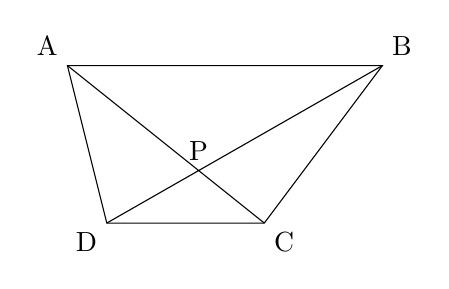
\begin{tikzpicture}[scale=1]
  \coordinate (A) at (0,2);
  \coordinate (B) at (4,2);
  \coordinate (D) at (0.5,0);
  \coordinate (C) at (2.5,0);
  \draw (A)--(B)--(C)--(D)--cycle;
  \draw (A)--(C) (B)--(D);
  % Robust intersection of diagonals for P
  \path[name path=ACline] (A)--(C);
  \path[name path=BDline] (B)--(D);
  \path[name intersections={of=ACline and BDline, by=P}];
  \node[above left] at (A) {A};\node[above right] at (B) {B};\node[below right] at (C) {C};\node[below left] at (D) {D};
  \node[above] at (P) {P};
\end{tikzpicture}
\end{center}

\begin{steps}
  \item \textbf{Part (i):} Consider $\triangle APB$ and $\triangle CPD$.
  \item Since AB $\parallel$ DC, $\angle PAB = \angle PCD$. \reason{alternate interior angles}
  \item Similarly, $\angle PBA = \angle PDC$. \reason{alternate interior angles}
  \item Also, $\angle APB = \angle CPD$. \reason{vertically opposite angles}
  \item Therefore, $\triangle APB\sim\triangle CPD$. \reason{AAA similarity}
  \item \textbf{Part (ii):} From the similarity proved in part (i), the ratio of corresponding sides is equal.
  \item $\dfrac{PA}{PC} = \dfrac{PB}{PD} = \dfrac{AB}{CD}$.
  \item Taking the first two parts of the proportion: $\dfrac{PA}{PC}=\dfrac{PB}{PD}$.
  \item Cross-multiply to get $PA\cdot PD=PB\cdot PC$. \reason{algebra}
\end{steps}

\finalanswer{(i) The triangles are similar. (ii) The product equality is proved.}

\subsection*{Question 7}
\textbf{Question:} In parallelogram ABCD, P is a point on BC. DP is extended to meet AB extended at L. Prove: (i) DP:PL = DC:BL (ii) DL:DP = AL:DC.

\solutionheading
\given{Parallelogram ABCD, P on BC, L is the intersection of extended DP and extended AB.}
\toprove{(i) $\dfrac{DP}{PL} = \dfrac{DC}{BL}$; (ii) $\dfrac{DL}{DP} = \dfrac{AL}{DC}$.}

\begin{center}
\begin{tikzpicture}[scale=1.2]
  \coordinate (A) at (0,2);
  \coordinate (B) at (4,2);
  \coordinate (D) at (1.2,0);
  \coordinate (C) at (5.2,0);
  \draw (A)--(B)--(C)--(D)--cycle;
  \coordinate (P) at ($(B)!0.6!(C)$);
  \path[name path=lineAB] ($(A)!-0.5!(B)$) -- ($(A)!1.5!(B)$);
  \path[name path=lineDP] (D) -- ($(D)!1.8!(P)$);
  \path[name intersections={of=lineAB and lineDP, by=L}];
  \draw (D)--(L);
  \node[above] at (A) {A};\node[above] at (B) {B};\node[below] at (C) {C};\node[below] at (D) {D};\node[below] at (P) {P};\node[above] at (L) {L};
\end{tikzpicture}
\end{center}

\begin{steps}
  \item \textbf{Part (i):} Consider $\triangle DPC$ and $\triangle LPB$.
  \item Since AL is an extension of AB, and AB $\parallel$ DC, we have AL $\parallel$ DC.
  \item $\angle PDC = \angle PLB$ (or $\angle PL A$). \reason{alternate interior angles}
  \item $\angle PCD = \angle PBL$. \reason{alternate interior angles, since AD $\parallel$ BC}
  \item Therefore, $\triangle DPC \sim \triangle LPB$. \reason{AA similarity}
  \item The ratio of corresponding sides is $\dfrac{DP}{LP} = \dfrac{PC}{PB} = \dfrac{DC}{LB}$.
  \item From this, we get the required relation: $\dfrac{DP}{PL} = \dfrac{DC}{BL}$.
  \item \textbf{Part (ii):} Start with the result from part (i): $\dfrac{PL}{DP} = \dfrac{BL}{DC}$. \reason{inverting the ratio}
  \item Add 1 to both sides: $\dfrac{PL}{DP} + 1 = \dfrac{BL}{DC} + 1$. \reason{algebra}
  \item Combine terms: $\dfrac{PL+DP}{DP} = \dfrac{BL+DC}{DC}$.
  \item Since D, P, L are collinear, $PL+DP=DL$.
  \item Since A, B, L are collinear, $BL+AB=AL$. Also, $AB=DC$ in a parallelogram.
  \item Substitute these into the equation: $\dfrac{DL}{DP} = \dfrac{BL+AB}{DC} = \dfrac{AL}{DC}$.
\end{steps}

\finalanswer{Both proportions are proved.}

\subsection*{Question 8}
\textbf{Question:} In $\triangle ABC$, $\angle ABC=2\angle ACB$. The bisector of $\angle ABC$, BP, meets AC at P. Show:
(i) CB:BA = CP:PA (ii) $AB\cdot BC=BP\cdot CA$.

\solutionheading
\given{$BP$ bisects $\angle ABC$; $\angle ABC=2\angle ACB$.}
\toprove{(i) CB:BA = CP:PA; (ii) $AB\cdot BC=BP\cdot CA$.}

\begin{center}
\begin{tikzpicture}[scale=1.2]
  \coordinate (B) at (0,0);
  \coordinate (C) at (5,0);
  \coordinate (A) at (1.5,3);
  \draw (A)--(B)--(C)--cycle;

  % Simple construction: pick P on AC and draw BP
  \path (A) -- (C) coordinate[pos=0.6] (P);
  \draw (B)--(P);

  % Place the labels
  \node[left] at (A) {A};
  \node[below left] at (B) {B};
  \node[below right] at (C) {C};
  \node[above] at (P) {P};
\end{tikzpicture}
\end{center}

\begin{steps}
  \item \textbf{Part (i):}
  \item In $\triangle ABC$, BP is the bisector of angle $\angle B$.
  \item By the Angle Bisector Theorem, the bisector divides the opposite side in the ratio of the other two sides.
  \item Therefore, $\dfrac{CB}{BA} = \dfrac{CP}{PA}$. This is equivalent to CB:BA = CP:PA.
  \item \textbf{Part (ii):}
  \item Let $\angle ACB = y$. Then the given condition is $\angle ABC = 2y$.
  \item Since BP bisects $\angle ABC$, we have $\angle ABP = \angle PBC = y$.
  \item Now consider $\triangle BPC$. We have $\angle PBC = y$ and $\angle PCB = y$.
  \item Since two angles are equal, $\triangle BPC$ is an isosceles triangle with $BP = PC$.
  \item Now consider $\triangle ABC$ and $\triangle APB$.
  \item $\angle BAC = \angle PAB$ (Common Angle A).
  \item $\angle ACB = y$ and $\angle ABP = y$. So, $\angle ACB = \angle ABP$.
  \item Therefore, $\triangle ABC \sim \triangle APB$. \reason{AA similarity}
  \item The ratio of corresponding sides is $\dfrac{AB}{AP} = \dfrac{BC}{PB} = \dfrac{AC}{AB}$.
  \item From $\dfrac{BC}{PB} = \dfrac{AC}{AB}$, we cross-multiply to get $AB \cdot BC = PB \cdot AC$.
  \item Note: The question has $BP \cdot CA$, which is the same.
\end{steps}

\finalanswer{Both parts are proved.}


\end{document}
